\newpage


\chapter{ Guía de Usuario}
\label{chap:manual-usuario}

La aplicación RobotUI ha sido creada por Manuel López Urbina para el proyecto fin de carrera de la titulación de Ingeniería Informática de la Universidad de Cádiz.\\

Resulta de vital importancia consultar esta guía antes y/o durante la utilización de los diferentes elementos tanto hardware, robot de pruebas desarrollado, como software del presente proyecto ya 
que le proporcionará una guía paso a paso en el manejo correcto de la aplicación.\\

La resolución recomendada para la aplicación debe ser superior o igual a 1024x768 (Estándar XGA), aunque es adaptable a cualquier resolución debido a su diseño web responsive.\\

RobotUI ha sido elaborado con un claro propósito; el de  proporcionar a los usuarios un medio donde compartir sus dispositivos robóticos con el resto de usuarios. Esto es posible gracias a una serie de
herramientas desarrolladas para que, sin necesidad de tener grandes conocimientos en programación, puedan configurar un entorno para el manejo de sus proyectos robóticos y tener 
posibilidad de compartir sus dispositivos y experiencias con el resto de usuarios.\\

La particularidad de RobotUI es que el usuario propietario del robot tiene la posibilidad de permitir el manejo de sus dispositivos robóticos al resto de usuarios que él mismo considere de una 
manera controlada o, por otra parte, permitir que otros usuarios visualicen, como si de espectadores se tratase, el control que un determinado usuario realiza de un determinado robot.
Todo ello en tiempo real.\\

Por tanto, tras esta breve introducción en el ámbito de la aplicación, en este manual se describen los diferentes pasos a realizar para configurar sus dispositivos correctamente en el sistema
y abrirlo a toda una comunidad de usuarios. Además de tener abierto el acceso a otros muchos dispositivos de otras personas.\\

\subsection{Objetivo de esta guía}

Esta guía tiene como objetivo proporcionar al usuario un soporte de ayuda e iniciación a la utilización de RobotUI.\\

Esta sección comprende:\\

\begin{itemize}
 \item Introducción.
 \item Guía de acceso al código fuente de la aplicación.
 \item Guía de uso de la aplicación.
 \item Guía para la puesta en marcha y programación de un robot.
\end{itemize}

\subsection{Dirigido a}

Esta guía esta dirigida al usuario final del proyecto SensorRS. Tiene la finalidad de proporcionar una guía descriptiva de los procedimientos de creación, configuración y utilización de los diferentes dispositivos 
robóticos en sus dos modalidades disponibles, la de control y la de visualización.

\subsection{Obtener SensorRS}

El código fuente junto con la presente memoria se encuentra disponible en el repositorio GitHub en el enlace \url{https://github.com/lopomaster/SensorRS} o usando la herramienta
Git, escribiendo en la consola el siguiente comando:\\

\begin{lstlisting}[language=bash]
 git clone git@github.com:lopomaster/SensorRS.git 
\end{lstlisting}


\section{ Uso de SensorRS }
\label{sec:uso-sensorrs}


\subsection{ Configuración }
\label{sec:configuracion}

Para la puesta en funcionamiento es necesario establecer una series de configuraciones en el código del robot con la finalidad de conectarlo a la aplicación RobotUI.\\

El manual de usuario de RobotUI se encuentra accesible en el respositorio del proyecto localizado en \url{ https://github.com/lopomaster/SAILS-RobotUI }
Para acceder a la aplicación, el usuario deberá acceder al siguiente enlace: \url{www.robotui.com}. \\

Al acceder podrá ver el portal de entrada a la aplicación. En él puede acceder al resto de funcionalidades identificándose con sus credenciales y acceder a los formularios de registro
de usuario.\\

\begin{figure}[H]
  \begin{center}
    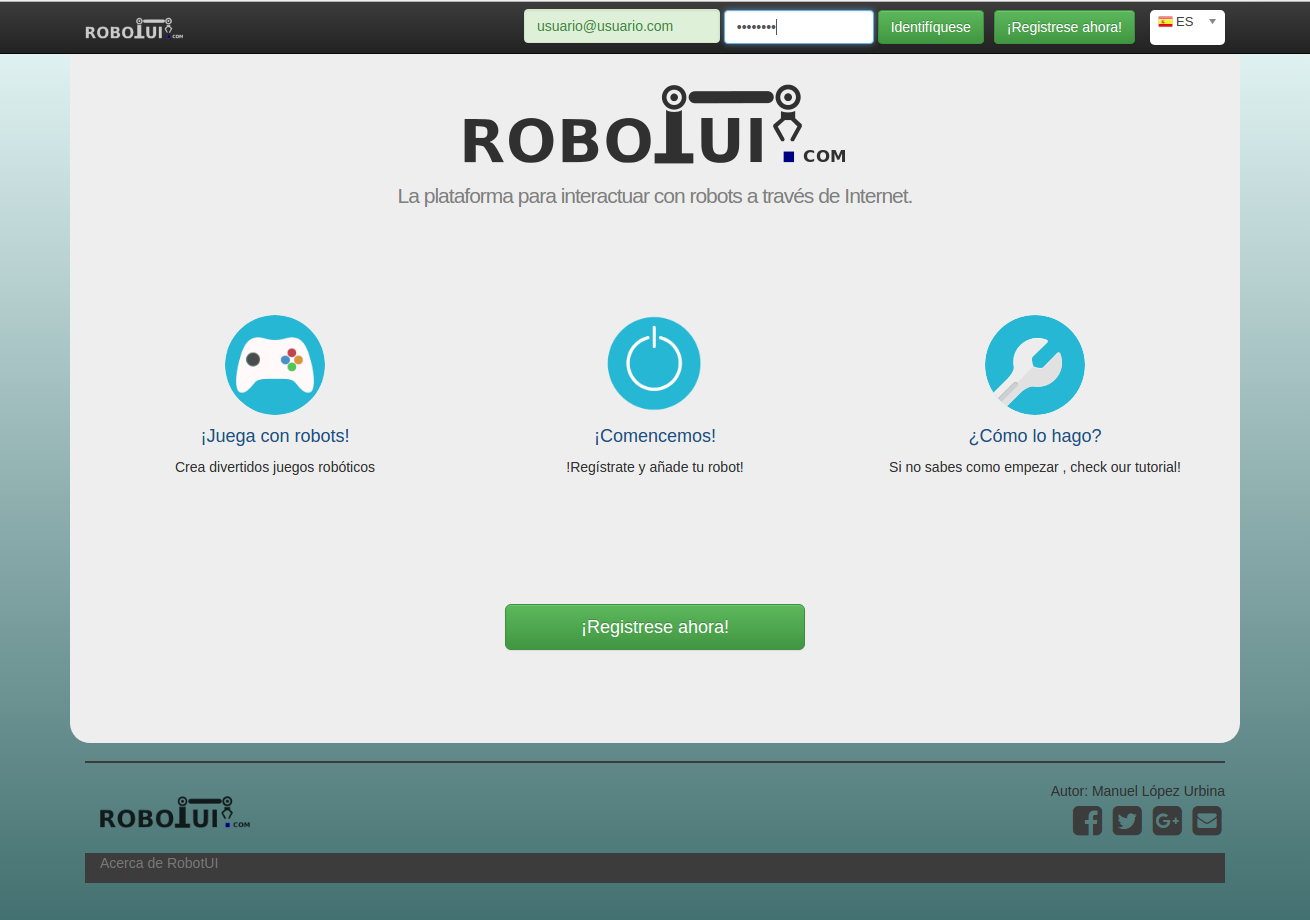
\includegraphics[scale=0.3]{imagenes/manual-usuario/pagina-principal.png}
  \end{center}
  \caption{Página principal RobotUI.}
  \label{website:pagina-principal}
\end{figure}


\subsection{ Programa tu robot }
\label{sec:programacion-robot}

NOTA: Esta guía comprende una serie de pasos para realizar la programación de un dispositivo robótico para la aplicación RobotUI. En este caso particular, el robot empleado posee como base una placa 
Raspberry Pi, la cual emplea para la conexión de sensores y motores haciendo uso de su sistema de Entrada/Salida Gpio.\\

El sistema es compatible con cualquier dispositivo, no solo limitado a las placas Raspberry. La única diferencia radica en que se deberán emplear a nivel de programación las bibliotecas adecuadas 
para la activación o lectura de las Entadas/Salidas correspondientes al modelo de placa utilizado.\\

Antes de proceder con la programación de nuestro robot debemos de realizar su creación en la aplicación RobotUI como queda descrito en el punto \ref{sec:creacion-robot} y 
tomar nota del identificador único que la aplicación proporciona para dicho robot y que posteriormente necesitaremos.\\	

\begin{figure}[H]
  \begin{center}
    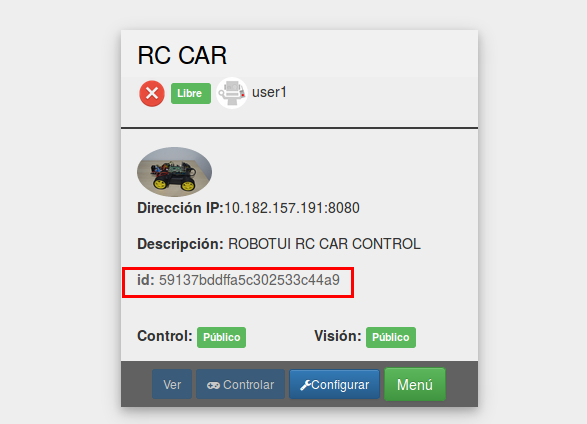
\includegraphics[scale=.6]{imagenes/manual-usuario/identificador.png}
  \end{center}
  \caption{Panel informativo de un robot donde se aprecia su identificador.}
  \label{website:pagina-principal}
\end{figure}

Una vez creado el robot y configurada su interfaz, añadiendo los diferentes elementos disponibles como acciones, vídeo, etiquetas, etcétera, recogidos en el punto \ref{subsec:configuracion-interfaz}: Configuración de la interfaz.
Podemos comenzar con la programación del robot.\\

Para ello debemos seguir una serie de pasos:\\

\begin{enumerate}
  \item Generar una archivo de extensión .js, con el código base mostrado en el punto \ref{codigo:base}.
  \item Reemplazar en el código la palabra \emph{IDENTIFICADOR} por el identificador único de nuestro robot obtenido en la vista informativa del mismo.
  Por ejemplo: 59188631c8e94ba54f7a4bdc.
  \item Indicar el puerto en el que el robot permanecerá a la escucha. Para ello debemos reemplazar palabra \emph{PUERTO} del código inferior por el puerto deseado. Por ejemplo 8085. 
  \item El siguiente paso es es determinar qué puertos GPIO necesitaremos y si van a ser utilizado en modo Entrada, Salida o Entrada/Salida dentro de la sección \emph{PINES} de la plantilla.
  En este caso se ha empleando la biblioteca \emph{pigpio} cuya documentación se encuentra disponible en el siguiente enlace: \url{https://www.npmjs.com/package/pigpio}.
  \item Definir el funcionamiento de los diferentes eventos dentro de la sección \emph{EVENTOS}.
\end{enumerate}


\subsubsection{código base}
\label{codigo:base}

\begin{lstlisting}[language=JavaScript]

var io_client = require('./node_modules/socket.io-client');
var sails_client = require('./node_modules/sails.io.js');
var io_server = sails_client(io_client);
io_server.sails.url = 'http://46.101.102.33:80';
io_server.socket.get('/robot/changetoonline/', {robot: 'IDENTIFICADOR', online: true});

// Inicia servidor socket.io en el puerto PUERTO.
var io =io_client.listen( PUERTO, { log: false });

var ffmpeg_command, running_camera = false, child_process = require('child_process');

var Gpio = require('pigpio').Gpio;


// SECCION PINES 

// EJEMPLO: 
//      var gpio2 = new Gpio(2, {mode: Gpio.OUTPUT}),
//	    gpio3 = new Gpio(3, {mode: Gpio.OUTPUT}),
//	    gpio17 = new Gpio(17, {mode: Gpio.OUTPUT}),
//	    gpio27 = new Gpio(27, {mode: Gpio.OUTPUT});


// FIN SECCION PINES


console.log('Esperando conexión...');

var sockets = {};

io.sockets.on('connection', function (socket)
{

    // SECCION EVENTOS

    // FIN SECCION EVENTOS
});

function stopStreaming(socket) {
  delete sockets[socket.id];
  // no more sockets, kill the stream
  if (Object.keys(sockets).length == 0) {
    if (ffmpeg_command){
      ffmpeg_command.kill();
      running_camera = false;
      console.log('Stop streaming');
    }
  }
}

function startStreaming(socket) {
  if (running_camera == false){
    console.log('Starting streaming....');
    var args = ["-f", "video4linux2", "-i", "/dev/video0", "-s", "300x150","-f","mjpeg", "pipe:1", "-b:v 28k", "-bufsize 28k"]
    ffmpeg_command = child_process.spawn("ffmpeg", args);
    running_camera = true
  }

  ffmpeg_command.on('error', function(err, stdout, stderr) {
    console.log("ffmpeg stdout:\n" + stdout);
    console.log("ffmpeg stderr:\n" + stderr);
    running_camera = false
  });


  ffmpeg_command.on('close', function (code) {
    console.log('ffmpeg exited' + code );
    running_camera = false
  });


  ffmpeg_command.stderr.on('data', function (data) {
    //console.log('stderr: ' + data);
  });

  ffmpeg_command.on('end', function() {
    console.log('Fin');
    running_camera = false
  });

  ffmpeg_command.stdout.on('data', function (data) {
    //console.log('stdout: ' + data);
    var frame = new Buffer(data).toString('base64');
    socket.emit('canvas',frame);
  });

}

\end{lstlisting}

A continuación mostramos dos posibles eventos para añadir al código base superior a modo orientativo:\\

El primer fragmento de cógigo se activa al recibir un evento tipo \emph{action} (evento lanzado desde la interfaz al presionar cualquier botón generado por el usuario), captura el comando recibido,
y si es igual a \emph{UP}, entonces habilita el pin gpio1 con el valor 1. Pin inicializado previamente en la sección de pines del código base.\\

\begin{lstlisting}[language=JavaScript]

socket.on('action', function (data){
    if (data == 'UP') {
        gpio1.digitalWrite(1);
    }
});

\end{lstlisting}

El segundo fragmento de código devuelve la lectura del pin \emph{gpio2} cada vez que recibe el comando \emph{READ} y mandando al cliente el valor de lectura obtenido:\\

\begin{lstlisting}[language=JavaScript]

  socket.on('action', function (data){
      if (data == 'READ') {
	var temp =  gpio2.digitalRead(1);
	socket.emit('robot_temp', {msg: temp});
    }
  });
\end{lstlisting}
 

En la parte referente a la interfaz de control de la aplicación RobotUI, para lanzar o capturar los comandos correspondientes a los ejemplos superiores, en el primer caso, debemos crear un botón 
cuyo código a emitir sea \emph{UP} y para el segundo, debemos añadir un botón cuyo código de emisión sea \emph{READ} y una etiqueta cuyo nombre de evento se corresponda con \emph{robot\_temp}.\\

Una vez generado el código para nuestro robot debemos copiarlo a la placa Raspberry Pi o computador que actuará como Robot para nuestra aplicación y ejecutarlo. Para la ejecución del código
introducimos el siguiente comando:\\

\begin{lstlisting}[language=bash]
  sudo node raspberry.js
\end{lstlisting}

Siendo \emph{raspberry.js} el nombre del archivo que contiene nuestro código.

Obteniendo el siguiente resultado:

\begin{figure}[H]
  \begin{center}
    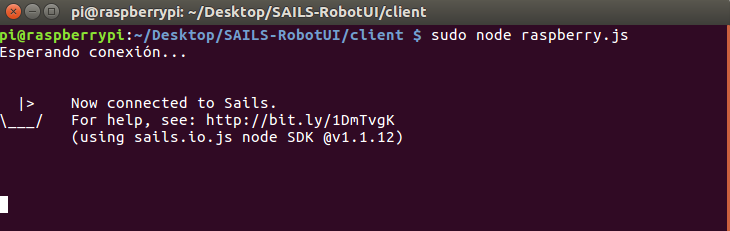
\includegraphics[scale=.6]{imagenes/manual-usuario/espera-conexion.png}
  \end{center}
  \caption{ Robot a la espera de conexión entrante.}
  \label{website:pagina-principal}
\end{figure}

